\section{Einleitung}
	\label{sec:einleitung}
	
	Greifen Kr"afte auf die Oberfl"ache eines K"orpers
	an, k"onnen diese Gestalts- oder Volumenver"anderungen hervorrufen. Diese wird auf die Fl"acheneinheit bezogen und die erhaltene physikalische Gr"o"se wird als Spannung bezeichnet.
	In Festk"orpern findet sich meist ein linearer Zusammenhang zwischen Deformation und Spannung, welcher durch der Elastizit"atsmodul gegeben ist. In diesem Versuch soll dieser f"ur verschiedene Metalle beestimmt werden.

\section{Theorie}
	\label{sec:theorie}

	\subsection{Spannung} % (fold)
	\label{sub:spannung}
	
		Spannung besitzt eine Tangential- und eine Normalkomponente. Die Normalkompomente wird als Normalspannung $\sigma$ oder auch Druck bezeichnet, w"ahrend die Tangentialkomponente Schubspannung genannt wird.

	\subsection{Hook'sches Gesetz} % (fold)
	\label{sub:hook_sches_gesetz}
	
		Ist die Deformation durch den Druck hinreichend klein, so findet sich meist ein linearer Zusammenhang zwischen der realtiven "Anderung $\delta L/L$ und der angreifenden Spannung $\sigma$. Es gilt:

		\begin{equation}
			\sigma = E \frac{\delta L}{L}
		\end{equation}

		Der Proportionalit"atsfaktor E wird als Elastizit"atsmodul bezeichnet und ist eine wichtige Materialkonstante.
		Eine einfache Methode dieses zu Messen ist die Methode der elastischen Biegung.

	\subsection{Zusammenhang des Elastizit"atsmoduls und der Schallgeschwindigkeit} % (fold)
	\label{sub:der_elastizit_atsmodul}

	\begin{figure}[!h]
		\centering
		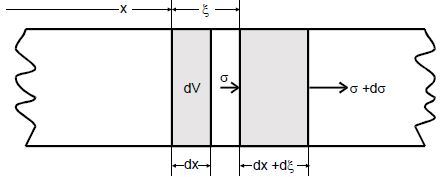
\includegraphics[width = 7cm]{img/schall.JPG}
		\caption{Skizze zur Ableitung eines Zusammenhanges zwischen Elastizit"atsmodul und Schallgeschwindigkeit. \cite{anleitung}}
		\label{fg:schall}
	\end{figure}
	
		Es besteht ein einfacher Zusammenhang zwischen dem Elastizit"asmodul $E$ und der Schallgeschwindikeit $c$. Durch einen Sto"s auf einer Stirnseite tritt eine sich longitudinal ausbreitende Deformation auf. Daher tritt eine ortsabh"angige Spannung $\sigma(x)$ auf. Es gilt daher hier:

		\begin{equation}
			\sigma = E \frac{\partial \eta}{\partial x}
		\end{equation}

		Daraus ergibt sich, nach der zeitlichen und r"aumlichen Verschiebung eines Volumenelements durch die Wellengleichung, f"ur die Schallgeschwindigkeit $c$:

		\begin{equation}
			c = \sqrt{\frac{E}{\rho}}
		\end{equation}

		Dabei ist $E$ der Elastizit"atsmodul und $\rho$ die Dichte des Stabes.

	\subsection{Berechnung der Durchbiegung eines homogenen Stabes bei einseitiger Einspannung} % (fold)
	\label{sub:1}
	
		\begin{wrapfigure}{i}{8cm}
			\centering
			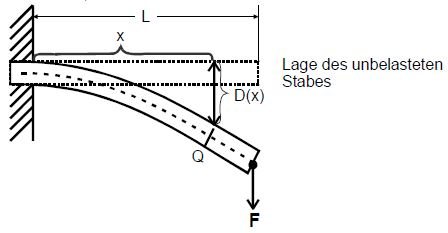
\includegraphics[width = 6.7cm]{img/biegung.JPG}
			\caption{Durchbiegung eines elastischen Stabes bei einseitiger Einspannung. \cite{anleitung}}
			\label{fg:biegung}
		\end{wrapfigure}

		Auf einen Stab greift eine Kraft wie in Abb. \ref{fg:biegung} an. Der Stab wird gebogen und die Durchbiegung $D(x)$ kann abgelesen werden. Durch eine Messreihe, in der die Gr"o"sen $D$ und $x$ gemessen werden, kann der Elastizit"atsmodul berechnet werden.

		Bei dieser Versuchsanordnung treten Kr"aftepaare auf, sodass eine Drehmomentgleichung aufgestellt werden muss, da ein Drehmoment $M_\mathrm{F}$ den Querschnitt $Q$ aus seiner vertikalen Lage verdreht. Im K"orper bilden sich nun Normalspannungen aus, welche der Deformation entgegenwirken. Auf der oberen Schicht ist dies die Zugspannung und in der unteren die Druckspannung. 

		\begin{wrapfigure}{r}{7cm}
			\centering
			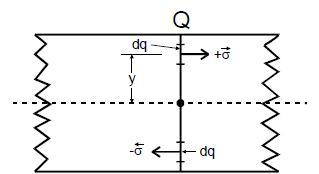
\includegraphics[width = 7cm]{img/berechnung.JPG}
			\caption{Skizze zur Berechnung des Drehmomentes $M_\mathrm{\sigma}$.\cite{anleitung}}
			\label{fg:berechnung}
		\end{wrapfigure}

		Zwischen diesen Fl"achen befindet sich die neutrale Faser, in der keine Spannungen auftreten. Diese ist in Abb. \ref{fg:biegung} als gestrichelte Linie dargestellt. An diesem Punkt ist die Zugspannung entgegengesetzt gleich der Druckspannung. Es bildet sich ein Drehmoment $M_\mathrm{\sigma}$ aus.
		Dieses ist im Falle der einseitigen Einspannung durch die "au"sere Kraft gegeben, welche "uber den Hebelarm $L-x$ angreift.

		\begin{equation}
			M_\mathrm{\sigma} = \int_Q y \sigma(y)\mathrm{d}q = F(L-x)
		\end{equation}

		$y$ ist dabei gleich dem Abstand von $\mathrm{d}q$ zur neutralen Faser. Aus der differentialgeometrie ergibt sich f"ur gro"se R eine Beziehung f"ur $1/R$. Wird das Hook'sche Gesetzt nun auf unser Problem angewendet ver"andert sich die Gleichung f"ur das Drehmoment zu:

		\begin{equation}
			E \frac{\mathrm{d}^2D}{\mathrm{d}x^2} \int_Q y^2 \mathrm{d} = F (L-x)
		\end{equation}

		Das Integral in dieser Gelchung wird als Fl"achentr"agheitsmoment $I$ bezeichnet: 

		\begin{equation}
			I = \int_Q y^2 \mathrm{d}
		\end{equation}

		Somit ergibt sich f"ur die Durchbiegung $D(x)$:

		\begin{equation}
			D(x) = \frac{F}{2EI} \left( Lx^2- \frac{x^3}{3} \right)
		\end{equation}

	\subsection{Berechnung der Durchbiegung eines homogenen Stabes bei zweiseitiger Auflage} % (fold)
	\label{sub:2}

	\begin{figure}[!h]
		\centering
		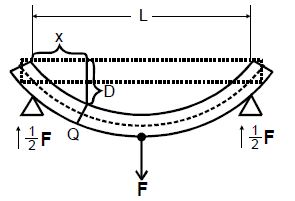
\includegraphics[width = 7cm]{img/biegung2.JPG}
		\caption{Durchbiegung eines homogenen Stabes bei zweiseitiger Auflage.}
		\label{fg:biegung2}
	\end{figure}

	Diesmal ist der Stab wie in Abb. \ref{fg:biegung2} eingespannt. In diesem Fall greift die Kraft $F/2$ mit dem Hebelarm $x$ an der Querschnittsfl"ache $Q$ an. 

	Da nun die Bereiche $0 \leq x \leq L/2$ und $L/2 \leq x \leq L$ getrennt betrachtet werden m"ussen, ergibt sich nach zweifacher Integration und Bestimmung der 1. konstanten durch annahme einer horitontalen Tangente an der Biegekurve  f"ur die Durchbiegung:

	\begin{eqnarray}
		D(x) &=& \frac{F}{48EI}(3L^2x-4x^3) , 0 \leq x \leq \frac{L}{2} \\
		D(x) &=& \frac{F}{48EI}(4x^3-12Lx^2+9L^2x-L^3) , \frac{L}{2} \leq x \leq L
	\end{eqnarray}

